\ifdefined\PRESENTATION\else\PassOptionsToClass{handout}{beamer}\fi\documentclass[aspectratio=169, lualatex]{beamer}
\makeatletter\def\input@path{{theme/}}\makeatother\usetheme{cipher}

\title{Applied Cryptography - 1.2: The Provable Security Mindset}
\author{Nadim Kobeissi}
\subject{Introduction to the One-Time Pad cipher and the provable security mindset in cryptography, covering XOR operations, security proofs, adversary models, and limitations of formal security analysis.}
\keywords{one-time pad, OTP, provable security, XOR, encryption, security proofs, Kerckhoffs' principle, cryptographic oracles, adversary models}
\institute{Symbolic Software}
\instituteimage{images/symbolicsoft-white.png}
\date{\today}
\coversubtitle{Summer 2026}
\coverpartname{Part 1: Provable Security}
\covertopicname{1.2: The Provable Security Mindset}
\coverwebsite{https://appliedcryptography.page}

\begin{document}
\begin{frame}[plain]
	\titlepage
\end{frame}

\section{Math Review}

\begin{frame}{Logs \& exponents}
	\begin{itemize}[<+->]
		\item Key identities to remember:
		      \begin{align*}
			      (x^a)(x^b) & = x^{a+b}             \\
			      (x^a)^b    & = x^{ab}              \\
			      \log_x(ab) & = \log_x a + \log_x b
		      \end{align*}
		\item \alert{Never write $(x^a)(x^b) = x^{ab}$!}
		\item Why we care: an $n$-bit key has $2^n$ possible values, and one more bit \emph{doubles} them: $2^{n+1} = 2 \cdot 2^n$.
	\end{itemize}
\end{frame}

\begin{frame}{Modular arithmetic}{Key definitions}
	\begin{itemize}[<+->]
		\item \textbf{Integers}: $\mathbb{Z} = \{\ldots, -2, -1, 0, 1, 2, \ldots\}$
		\item \textbf{Natural numbers}: $\mathbb{N} = \{0, 1, 2, \ldots\}$
		\item \textbf{Divides}: $n \mid x$ means $x = kn$ for some integer $k$
		\item \textbf{Example}: $7 \mid 84$ because $84 = 12 \cdot 7$
	\end{itemize}
\end{frame}

\begin{frame}{The modulo operation}
	\begin{itemize}[<+->]
		\item $a \bmod n$ gives the remainder when dividing $a$ by $n$
		\item Result is always in $\{0, 1, \ldots, n-1\}$
		\item We call this set $\mathbb{Z}_n = \{0, 1, \ldots, n-1\}$ (it comes back at the end of the lecture)
		\item \textbf{Even for negative numbers!}
		      \begin{align*}
			      21 \bmod 7  & = 0                          \\
			      20 \bmod 7  & = 6                          \\
			      -20 \bmod 7 & = 1 \quad \text{(not $-6$!)}
		      \end{align*}
		\item Think: ``$a$ is $(a \bmod n)$ more than a multiple of $n$''
	\end{itemize}
\end{frame}

\begin{frame}{Understanding modulo with clocks}
	\begin{columns}[c]
		\column{0.5\textwidth}{
			\begin{itemize}[<+->]
				\item Clock arithmetic is modulo 12
				\item 15:00 = 3:00 PM because $15 \bmod 12 = 3$
				\item 7 hours after 9:00?
				      \begin{itemize}[<+->]
					      \item $(9 + 7) \bmod 12 = 16 \bmod 12 = 4$
				      \end{itemize}
				\item 5 hours before 2:00?
				      \begin{itemize}[<+->]
					      \item $(2 - 5) \bmod 12 = -3 \bmod 12 = 9$
				      \end{itemize}
				\item The clock face is $\mathbb{Z}_{12}$ in disguise: its ``12'' is our $0$
			\end{itemize}
		}
		\column{0.5\textwidth}{
			\begin{center}
				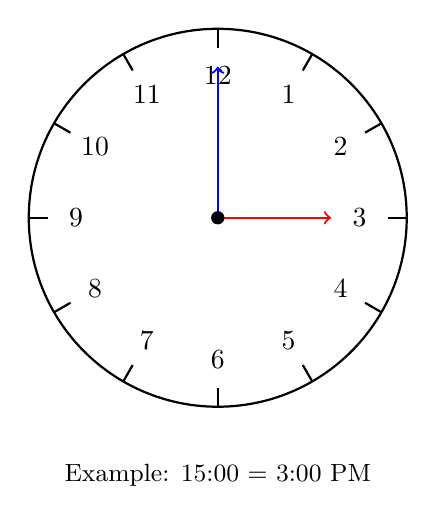
\begin{tikzpicture}[scale=1.2]
					\draw[thick] (0,0) circle (2cm);
					\foreach \hour in {1,2,...,12} {
							\pgfmathsetmacro{\angle}{90 - \hour * 30}
							\draw[thick] (\angle:1.8cm) -- (\angle:2cm);
							\node at (\angle:1.5cm) {\hour};
						}
					\draw[thick, ->, red] (0,0) -- (0:1.2cm);
					\draw[thick, ->, blue] (0,0) -- (90:1.6cm);
					\fill (0,0) circle (2pt);
					\node[below] at (0,-2.5cm) {\small Example: 15:00 = 3:00 PM};
				\end{tikzpicture}
			\end{center}
		}
	\end{columns}
\end{frame}

\begin{frame}{Binary strings}
	\begin{itemize}[<+->]
		\item $\bits^n$ = set of $n$-bit binary strings
		\item $|x|$ = length of string $x$
		\item $\bit{0}^n$ = string of $n$ zeros, $\bit{1}^n$ = string of $n$ ones
		\item $|\bits^n| = 2^n$: there are $2^n$ such strings, e.g.\ $\bits^2 = \{\bit{00}, \bit{01}, \bit{10}, \bit{11}\}$
	\end{itemize}
\end{frame}

\begin{frame}{Probability basics}
	\begin{itemize}[<+->]
		\item \textbf{Distribution}: assigns a probability to each outcome
		\item For each outcome $x$: $0 \leq \Pr[x] \leq 1$
		\item Sum of all probabilities = 1
		\item \textbf{Uniform distribution}: $\Pr[x] = \frac{1}{|\mathcal{X}|}$ for all $x \in \mathcal{X}$
		      \begin{itemize}
			      \item $\frac{1}{|\mathcal{X}|}$ means ``one divided by the size of set $\mathcal{X}$''
			      \item Example: Rolling a fair die has a uniform distribution with $\Pr[x] = \frac{1}{6}$ for each outcome
		      \end{itemize}
		\item Basic fact: $\Pr[A] = 1 - \Pr[\neg A]$
		      \begin{itemize}
			      \item $\neg A$ means ``not A''
			      \item All outcomes where $A$ does not occur
		      \end{itemize}
	\end{itemize}
\end{frame}

\begin{frame}{Notation in pseudocode}
	\begin{itemize}[<+->]
		\item $x \twoheadleftarrow \mathcal{X}$: sample $x$ uniformly from set $\mathcal{X}$
		\item $x \coloneq 5$: assign value $5$ to variable $x$
		\item $x \stackrel{?}{=} y$: check if $x$ equals $y$ (returns true/false)
	\end{itemize}
\end{frame}

\section{The Provable Security Mindset}

\begin{frame}{How it's made}
	\bigimagewithcaption[0.9\textwidth]{fischer-theory.png}{Fischer et al., The Challenges of Bringing Cryptography from Research Papers to Products: Results from an Interview Study with Experts, USENIX Security 2024}
\end{frame}

\begin{frame}{Thinking about secrecy}{Attempt 1: keep the whole design secret}
	\bigimagewithcaption[0.97\textwidth]{naive-enc.pdf}{Source: The Joy of Cryptography}
\end{frame}

\begin{frame}{Thinking about secrecy}{Attempt 1: keep the whole design secret}
	\begin{columns}[c]
		\column{0.5\textwidth}{
			\begin{itemize}[<+->]
				\item Keep the whole design secret?
				\item \textbf{``Advantages''}:
				      \begin{itemize}[<+->]
					      \item Attacker doesn't know how our cipher (or system, more generally) works.
				      \end{itemize}
				\item \textbf{Disadvantages}:
				      \begin{itemize}[<+->]
					      \item Figuring out how the system works might mean a break.
					      \item Can't expose cipher to scrutiny.
					      \item Everyone needs to invent their own cipher.
				      \end{itemize}
			\end{itemize}
		}
		\column{0.5\textwidth}{
			\imagewithcaption{naive-enc.pdf}{Source: The Joy of Cryptography}
		}
	\end{columns}
\end{frame}

\begin{frame}{Kerckhoffs' principle}{Reminder}
	\begin{itemize}[<+->]
		\item \textit{``A cryptosystem should be secure even if everything about the system, except the key, is public knowledge.''} --- Auguste Kerckhoffs, 1883
		\item \textbf{Why it matters}:
		      \begin{itemize}[<+->]
			      \item No ``security through obscurity''
			      \item The key is the only secret: the rest can be audited, tested, trusted
			      \item Encourages open standards and peer review
			      \item If your system's security depends on nobody knowing how it works, it's not secure.
		      \end{itemize}
	\end{itemize}
\end{frame}

\begin{frame}{Thinking about secrecy}{Attempt 2: keep only the key secret}
	\bigimagewithcaption[0.97\textwidth]{keyed-enc.pdf}{\textbf{Concentrate all the need for secrecy in the key!}}
\end{frame}

\begin{frame}{Thinking about secrecy}{Attempt 2: keep only the key secret}
	\begin{columns}[c]
		\column{0.5\textwidth}{
			\begin{itemize}[<+->]
				\item Cipher can be scrutinized and used by anyone.
				\item Security can be shown to hold so long as the key is secret.
				\item This is how virtually all cryptography is designed today.
			\end{itemize}
		}
		\column{0.5\textwidth}{
			\imagewithcaption{keyed-enc.pdf}{Source: The Joy of Cryptography}
		}
	\end{columns}
\end{frame}

\begin{frame}{One-time pad}{First look at a symmetric cipher}
	\begin{columns}[c]
		\begin{column}{0.5\textwidth}
			\sssubroutine{Enc}{K, M}{
				$C \coloneq K \oplus M$ \\
				return $C$
			}{2}
		\end{column}
		\begin{column}{0.5\textwidth}
			\sssubroutine{Dec}{K, C}{
				$M \coloneq K \oplus C$ \\
				return $M$
			}{2}
		\end{column}
	\end{columns}
	\vspace{0.5em}
	\begin{center}
		$K, M \in \bits^n$: the key is exactly as long as the message, $|K| = |M|$. Remember this.
	\end{center}
\end{frame}

\begin{frame}{The XOR (exclusive OR) operation}
	\begin{columns}[c]
		\column{0.6\textwidth}{
			\begin{center}
				\begin{tabular}{|c|c|c|}
					\hline
					\textbf{A} & \textbf{B} & \textbf{A $\oplus$ B} \\
					\hline
					\bit{0}    & \bit{0}    & \bit{0}               \\
					\hline
					\bit{0}    & \bit{1}    & \bit{1}               \\
					\hline
					\bit{1}    & \bit{0}    & \bit{1}               \\
					\hline
					\bit{1}    & \bit{1}    & \bit{0}               \\
					\hline
				\end{tabular}
			\end{center}
			\begin{itemize}
				\item \bit{1} when the inputs differ, \bit{0} when they agree
				\item On strings, bit by bit: $\bit{0110} \oplus \bit{1100} = \bit{1010}$
				\item Commutative and associative: reorder and regroup freely
				\item $x \oplus x = \bit{0}$ and $x \oplus \bit{0} = x$, so $(M \oplus K) \oplus K = M$
			\end{itemize}
		}
		\column{0.4\textwidth}{
			\begin{center}
				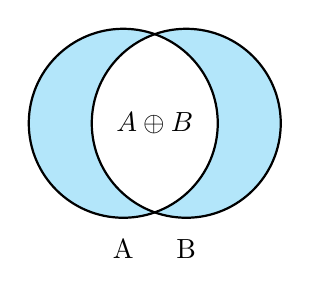
\begin{tikzpicture}[scale=0.8]
					\fill[cyan!30] (0,0) circle (1.5);
					\fill[cyan!30] (1,0) circle (1.5);
					\begin{scope}
						\clip (0,0) circle (1.5);
						\fill[white] (1,0) circle (1.5);
					\end{scope}
					\draw[thick] (0,0) circle (1.5);
					\draw[thick] (1,0) circle (1.5);
					\node at (0,-2) {A};
					\node at (1,-2) {B};
					\node at (0.5,0) {$A \oplus B$};
				\end{tikzpicture}
			\end{center}
		}
	\end{columns}
\end{frame}

\begin{frame}{One-time pad}{First look at a symmetric cipher}
	\bigimagewithcaption[0.97\textwidth]{xor-enc.png}{(We're encoding the message and key as bits)}
\end{frame}

\begin{frame}{One-time pad}{First look at a symmetric cipher}
	\bigimagewithcaption[0.97\textwidth]{xor-dec.png}{(We're encoding the message and key as bits)}
\end{frame}

\begin{frame}{Where does the key come from?}{Sampling $K$ uniformly}
	\begin{itemize}[<+->]
		\item The cipher is only as good as its key. How should the victim pick $K$?
		\item $K \twoheadleftarrow \bits^n$: sample $K$ \textbf{uniformly} from all $2^n$ possible $n$-bit strings.
		      \begin{itemize}
			      \item Every key has probability exactly $\frac{1}{2^n}$; no key is likelier than any other.
			      \item Nothing about $K$ can be predicted before it is sampled, not even a single bit.
		      \end{itemize}
		\item A \textbf{fresh} $K$ for every message. The name is a hint: one-\emph{time} pad.
		\item In practice, the operating system harvests unpredictable events (interrupt timings, hardware noise) and stretches them with a pseudorandom generator. That is topic 1.4.
		\item Today we \emph{assume} $K$ is truly uniform. Whether real machines deliver that is a separate question; we return to it at the end.
	\end{itemize}
\end{frame}

\begin{frame}{One-time pad}{Correctness proof}
	\begin{itemize}[<+->]
		\item \textbf{Claim}: $\forall n > 0,\; \forall K, M \in \bits^{n}:\; \textsf{Dec}(K, \textsf{Enc}(K, M)) = M$.\\
		      In words: decrypting with the same key always undoes encrypting.
		\item \textbf{Proof}:
		      \begin{align*}
			      \textsf{Dec}(K, \textsf{Enc}(K, M)) & = \textsf{Dec}(K, K \oplus M) && \textcolor{gray}{\small\text{definition of Enc}} \\
			                                          & = K \oplus (K \oplus M)       && \textcolor{gray}{\small\text{definition of Dec}} \\
			                                          & = (K \oplus K) \oplus M       && \textcolor{gray}{\small\text{associativity}}     \\
			                                          & = \bit{0}^n \oplus M          && \textcolor{gray}{\small x \oplus x = \bit{0}^n}   \\
			                                          & = M                           && \textcolor{gray}{\small \bit{0}^n \oplus x = x} \quad \qed
		      \end{align*}
	\end{itemize}
\end{frame}

\begin{frame}{One-time pad}{How do we prove security?}
	\begin{columns}[c]
		\begin{column}{0.5\textwidth}
			\begin{itemize}[<+->]
				\item A security proof says what an attacker can and cannot learn when they interact with the victim only through a fixed interface: \textsc{Attack}$(M)$.
				\item ``Victim'' chooses their key.
				      \begin{itemize}
					      \item Fresh key for each message (each key used only once)
				      \end{itemize}
				\item Adversary chooses the message and receives the ciphertext.
				\item We say that \textbf{the adversary has access to an encryption oracle}.
			\end{itemize}
		\end{column}
		\begin{column}{0.5\textwidth}
			\imagewithcaption{attacker-interface.pdf}{Source: The Joy of Cryptography}
		\end{column}
	\end{columns}
\end{frame}

\begin{frame}{One-time pad}{How do we prove security?}
	\begin{center}
		\begin{tikzpicture}[
				box/.style={rectangle, draw, minimum height=2.5cm, align=left, fill=white},
				dashed box/.style={rectangle, draw, dashed, minimum width=2.5cm, minimum height=2.5cm, align=center, fill=white},
				>=Stealth,
			]
			\node[dashed box] (adversary) {\textit{adversary}};
			\node[box, right=2cm of adversary](attack){
				$\underline{\func{attack}{M}}$: \hfill \quad \quad \textcolor{gray}{\scriptsize \textit{// adversary chooses $M$}} \\
				\quad $K \twoheadleftarrow \bits^{n}$ \hfill \quad \quad \textcolor{gray}{\scriptsize \textit{// victim samples $K$}} \\
				\quad $C \coloneq \textsf{Enc}(K, M)$ \hfill \quad \quad \textcolor{gray}{\scriptsize \textit{// victim encrypts}} \\
				\quad return $C$ \hfill \quad \quad \textcolor{gray}{\scriptsize \textit{// adversary sees $C$}}
			};
			\draw[->] (adversary) -- node[above] {$M$} (attack);
			\draw[<-] ([yshift=-0.5cm]adversary.east) -- node[below] {$C$} ([yshift=-0.5cm]attack.west);
		\end{tikzpicture}
	\end{center}
\end{frame}

\begin{frame}{One-time pad}{How do we prove security?}
	\begin{columns}[c]
		\begin{column}{0.55\textwidth}
			\begin{itemize}[<+->]
				\item Adversary can query the oracle an unbounded number of times.
				\item The same $M$ twice gives (almost always) different $C, C'$: fresh $K$ each time.
				\item $K$ is always sampled correctly: uniformly, by the victim.
				\item The oracle is \textbf{randomized}: its output depends on coins the attacker never sees.
				\item The attacker never sees $K$.
			\end{itemize}
		\end{column}
		\begin{column}{0.45\textwidth}
			\imagewithcaption{attacker-interface.pdf}{Source: The Joy of Cryptography}
		\end{column}
	\end{columns}
\end{frame}

\begin{frame}
	\begin{center}
		\Large\textit{``If I use OTP according to the attack scenario (I sample keys uniformly and use each key to encrypt just one message), then no matter how the plaintexts are chosen, and no matter how the ciphertext is subsequently used, I can enjoy a certain security guarantee.''}\\[1em]
		{\normalsize --- The Joy of Cryptography}
	\end{center}
\end{frame}

\begin{frame}{One-time pad}{How do we prove security?}
	\begin{columns}[c]
		\begin{column}{0.5\textwidth}
			\begin{itemize}[<+->]
				\item \textbf{Generally}: a cipher is secure if the adversary can't distinguish the output of calls to \textsc{Attack} from random junk.
				\item \textbf{Formally, for OTP}: for all positive integers $n$ and all choices of plaintext $M \in \bits^n$, the output of the following subroutine is uniformly distributed:
			\end{itemize}
		\end{column}
		\begin{column}{0.5\textwidth}
			\sssubroutine{Attack}{M}{
				$K \twoheadleftarrow \bits^{n}$ \\
				$C \coloneq K \oplus M$ \\
				return $C$
			}{1.5}
		\end{column}
	\end{columns}
\end{frame}

\begin{frame}{One-time pad}{How do we prove security?}
	\begin{columns}[c]
		\begin{column}{0.7\textwidth}
			\begin{itemize}[<+->]
				\item Claim: if $K$ is uniform, so is $C$. Let's check it by hand for $n = 2$.
				\item Suppose $M = \bit{01}$:
				      \begin{itemize}[<+->]
					      \item $K = \bit{00}$ (probability $1/4$): $C = \bit{00} \oplus \bit{01} = \bit{01}$.
					      \item $K = \bit{01}$ (probability $1/4$): $C = \bit{01} \oplus \bit{01} = \bit{00}$.
					      \item $K = \bit{10}$ (probability $1/4$): $C = \bit{10} \oplus \bit{01} = \bit{11}$.
					      \item $K = \bit{11}$ (probability $1/4$): $C = \bit{11} \oplus \bit{01} = \bit{10}$.
				      \end{itemize}
				\item Every $C \in \bits^2$ shows up exactly once, so $\Pr[C] = 1/4$ for each. Uniform!
			\end{itemize}
		\end{column}
		\begin{column}{0.3\textwidth}
			\sssubroutine{Attack}{M}{
				$K \twoheadleftarrow \bits^{n}$ \\
				$C \coloneq K \oplus M$ \\
				return $C$
			}{1.5}
		\end{column}
	\end{columns}
\end{frame}

\begin{frame}{One-time pad}{What's so special about XOR?}
	\begin{columns}[c]
		\begin{column}{0.7\textwidth}
			\begin{itemize}[<+->]
				\item Let's replace $\oplus$ with $\land$ (AND). What would happen?
				\item Output no longer uniform! Wherever $M$ has a \bit{0}, so does $C$, whatever $K$ is: $\textsc{Attack}(\bit{0}^n) = \bit{0}^n$ every time.
				\item XOR's trick: fix $M$ and read down its column. Every output appears exactly once, so uniform $K$ gives uniform $C$.
			\end{itemize}
			\begin{center}
				\small
				\begin{tabular}{|c|c|c|c|}
					\hline
					\textbf{K} & \textbf{M} & \textbf{K $\oplus$ M} & \textbf{K $\land$ M} \\
					\hline
					\bit{0}    & \bit{0}    & \bit{0}               & \bit{0}              \\
					\hline
					\bit{0}    & \bit{1}    & \bit{1}               & \bit{0}              \\
					\hline
					\bit{1}    & \bit{0}    & \bit{1}               & \bit{0}              \\
					\hline
					\bit{1}    & \bit{1}    & \bit{0}               & \bit{1}              \\
					\hline
				\end{tabular}
			\end{center}
		\end{column}
		\begin{column}{0.3\textwidth}
			\sssubroutine{Attack}{M}{
				$K \twoheadleftarrow \bits^{n}$ \\
				$C \coloneq K \land M$ \\
				return $C$
			}{1.5}
		\end{column}
	\end{columns}
\end{frame}

\begin{frame}{One-time pad}{How do we prove security?}
	\begin{columns}[c]
		\begin{column}{0.7\textwidth}
			\begin{itemize}[<+->]
				\item What if this is true only for $M = \bit{01}$?
				\item Fine, let's pick any $M, C \in \bits^n$.
				\item What is \prob{\textsc{Attack}(M) = C}?
				\item \textsc{Attack}$(M)$ returns $C$ exactly when $C = \textsf{Enc}(K, M) = K \oplus M$\ldots
				\item \ldots which occurs for exactly one key: $K = M \oplus C$.
				\item Since $K$ is chosen uniformly from $\bits^n$, the probability of choosing that $K$ is $\frac{1}{2^n}$.
				\item Same for every $C \in \bits^n$: all $2^n$ outputs are equally likely. That is what ``uniform'' means. $\qed$
			\end{itemize}
		\end{column}
		\begin{column}{0.3\textwidth}
			\sssubroutine{Attack}{M}{
				$K \twoheadleftarrow \bits^{n}$ \\
				$C \coloneq K \oplus M$ \\
				return $C$
			}{1.5}
		\end{column}
	\end{columns}
\end{frame}

\begin{frame}{One-time pad}{From the adversary's perspective\ldots}
	\begin{columns}[c]
		\begin{column}{0.35\textwidth}
			\sssubroutine{Attack}{M}{
				$K \twoheadleftarrow \bits^{n}$ \\
				$C \coloneq K \oplus M$ \\
				return $C$
			}{1.5}
		\end{column}
		\begin{column}{0.3\textwidth}
			\begin{center}
				{\huge{$\approxeq$}} \\[1em]
				{\scriptsize\textit{(indistinguishable \\ from)}}
			\end{center}
		\end{column}
		\begin{column}{0.35\textwidth}
			\sssubroutine{Junk}{M}{
				$C \twoheadleftarrow \bits^{n}$ \\
				return $C$
			}{2}
		\end{column}
	\end{columns}
\end{frame}

\begin{frame}
	\begin{center}
		\huge \textit{``Real or random?''}
	\end{center}
\end{frame}

\begin{frame}{One-time pad}{What about addition modulo $n$?}
	\begin{columns}[c]
		\begin{column}{0.58\textwidth}
			\begin{itemize}[<+->]
				\item Let's replace $\oplus$ with addition modulo $n$. What would happen? ($K, M, C \in \mathbb{Z}_n$ are now numbers, not bit strings.)
				\item Still good!
				\item Can you prove correctness and security?
				      \begin{itemize}[<+->]
					      \item Correctness: what is $\textsf{Dec}$? Remember $(2 - 5) \bmod 12 = 9$.
					      \item Security: how many $K \in \mathbb{Z}_n$ give $(K + M) \bmod n = C$, for fixed $M$ and $C$?
				      \end{itemize}
			\end{itemize}
		\end{column}
		\begin{column}{0.42\textwidth}
			\sssubroutine{Attack}{M}{
				$K \twoheadleftarrow \mathbb{Z}_{n}$ \\
				$C \coloneq (K + M) \bmod n$ \\
				return $C$
			}{1.5}
		\end{column}
	\end{columns}
\end{frame}

\section{Breaking One-Time Pads}

\begin{frame}{Two-time pads}{What happens when we reuse a key?}
	\begin{columns}[c]
		\column{1\textwidth}{
			\begin{itemize}[<+->]
				\item Alice sends two messages with the same key:
				\item $C_1 = M_1 \oplus K$
				\item $C_2 = M_2 \oplus K$
				\item What can Eve learn from $C_1$ and $C_2$?
				\item $C_1 \oplus C_2 = (M_1 \oplus K) \oplus (M_2 \oplus K)$
				\item $C_1 \oplus C_2 = M_1 \oplus M_2 \oplus (K \oplus K)$
				\item $C_1 \oplus C_2 = M_1 \oplus M_2$
				\item \alert{The key cancels out completely!}
			\end{itemize}
		}
	\end{columns}
\end{frame}

\begin{frame}{Exploiting $M_1 \oplus M_2$}{Why is this dangerous?}
	\begin{itemize}[<+->]
		\item Knowing $M_1 \oplus M_2$ allows statistical attacks:
		\item \textbf{Language patterns}: Natural language has predictable structure
		      \begin{itemize}[<+->]
			      \item Common words: ``the'', ``and'', ``of'', ``to''
			      \item Letter frequencies: E is most common in English (12.7\%)
			      \item Spaces are very frequent (about 18\% of characters), and in ASCII, letter $\oplus$ space just flips the letter's case: where $M_1 \oplus M_2$ looks like a letter, one message probably has a space
		      \end{itemize}
		\item \textbf{Crib dragging}: Try XORing common words at different positions
		\item \textbf{Example}: If we guess ``the'' at position $i$ in $M_1$:
		      \begin{itemize}[<+->]
			      \item Extract: $(M_1 \oplus M_2)[i:i+3] \oplus \text{``the''}$
			      \item If the result looks like valid text, we may have found part of $M_2$!
		      \end{itemize}
	\end{itemize}
\end{frame}

\begin{frame}{Malleability of one-time pads}{Another practical weakness}
	\begin{columns}[c]
		\column{1\textwidth}{
			\begin{itemize}[<+->]
				\item OTP provides confidentiality but not integrity
				\item \textbf{Malleability}: Attacker can modify ciphertext predictably
				\item Given $C = M \oplus K$
				\item Attacker creates $C' = C \oplus \Delta$
				\item Decryption: $C' \oplus K = (M \oplus K \oplus \Delta) \oplus K$
				\item Result: $M' = M \oplus \Delta$
				\item \alert{Attacker controls the change without knowing $M$ or $K$!}
			\end{itemize}
		}
	\end{columns}
\end{frame}

\begin{frame}{Malleability in practice}{Turning \$100 into \$900}
	\begin{itemize}[<+->]
		\item \textbf{Scenario}: Bank transfer message
		\item Original: ``Transfer \$0100.00 to Account 12345''
		\item Attacker knows position of amount field
		\item Flips a bit to change `1' (ASCII 49 = \texttt{00110001}) to `9' (ASCII 57 = \texttt{00111001})
		\item XOR difference: \texttt{00110001} $\oplus$ \texttt{00111001} = \texttt{00001000}
		\item Apply $\Delta$ = \texttt{00001000} at the correct position in the ciphertext
		\item Result: ``Transfer \$0900.00 to Account 12345''
		\item \alert{No need to break encryption or know the key!}
	\end{itemize}
\end{frame}

\begin{frame}{Discussion time}
	\begin{columns}[c]
		\begin{column}{0.68\textwidth}
			\begin{enumerate}
				\item \textbf{We proved OTP secure, then broke it twice. Which is wrong: the proof or the attacks?}
				      \begin{itemize}
					      \item Reread \textsc{Attack}$(M)$ line by line. Which line does the two-time pad violate? Which one does malleability violate?
				      \end{itemize}
				\item \textbf{Is malleability an attack on secrecy?}
				      \begin{itemize}
					      \item The attacker turned \$100 into \$900 without learning a single bit of $M$. What did our definition promise, and what did it never promise?
				      \end{itemize}
				\item \textbf{Would addition modulo $n$ have helped against either attack?}
			\end{enumerate}
		\end{column}
		\begin{column}{0.32\textwidth}
			\imagewithcaption{spamton-sez.png}{}
		\end{column}
	\end{columns}
\end{frame}

\section{Limitations of Security Proofs}

\begin{frame}{OTP: security assumptions \& constraints}{Part 1}
	\begin{itemize}[<+->]
		\item Our security proofs rely on specific assumptions about the adversary:
		      \begin{itemize}[<+->]
			      \item \textbf{Key reuse}: Keys are never intentionally reused (though may repeat by chance).
			      \item \textbf{Observation only}: Adversary passively observes the ciphertext but doesn't tamper with it.
			      \item \textbf{Message independence}: Choice of message $M$ is independent of key $K$.
			      \item \textbf{Key secrecy}: Adversary learns nothing about the key.
			      \item \textbf{No sampling influence}: Adversary cannot influence how the key is sampled.
		      \end{itemize}
		\item Each attack in the last section broke exactly one of these. The proof never claimed to survive that.
	\end{itemize}
\end{frame}

\begin{frame}{OTP: security assumptions \& constraints}{Part 2}
	\begin{itemize}[<+->]
		\item Side-channel attacks violate our model:
		      \begin{itemize}[<+->]
			      \item We assume the adversary cannot coerce the victim into running a different algorithm.
			      \item Cannot observe execution details:
			            \begin{itemize}[<+->]
				            \item CPU timing information (clock cycles).
				            \item Memory access patterns.
				            \item Cache hits/misses.
				            \item Power consumption during encryption.
			            \end{itemize}
		      \end{itemize}
		\item The proof covers exactly the interface of \textsc{Attack}$(M)$: one input in, one output out. Anything else the attacker can measure is outside the model, and the proof is silent about it.
	\end{itemize}
\end{frame}

\begin{frame}{Limitations of security proofs}{Part 1}
	\begin{itemize}[<+->]
		\item Rigor and the real world famously don't mix.
		\item Security proofs are good for rigor but say very little about real-world concerns:
		      \begin{itemize}[<+->]
			      \item How can Alice and Bob obtain a secret key that only they know?
			      \item How can they keep $K$ secret?
			      \item How can a computer sample from the uniform distribution?
			      \item How can Alice ensure that $C$ is sent reliably to Bob?
		      \end{itemize}
	\end{itemize}
\end{frame}

\begin{frame}{Limitations of security proofs}{Part 2}
	\begin{itemize}[<+->]
		\item More questions proofs don't address:
		      \begin{itemize}[<+->]
			      \item How can Alice hide the fact that she is talking to Bob (rather than hide only the content)?
			      \item How can Alice be sure that she is communicating with Bob, not an impostor?
			      \item How can we incentivize Alice and Bob to use encryption?
			      \item Should the government be allowed to obtain a warrant to read encrypted communications?
		      \end{itemize}
		\item A proof is a precise answer to a precise question: \emph{in this scenario, against this adversary, this property holds.}
		\item On every question above it is not wrong, just silent. Necessary, not sufficient.
	\end{itemize}
\end{frame}

\begin{frame}{Key distribution problem}{The elephant in the room}
	\begin{columns}[c]
		\column{0.6\textwidth}{
			\begin{itemize}[<+->]
				\item OTP needs a fresh key as long as the message. How do Alice and Bob share it?
				\item \textbf{The paradox}: if you can securely send the key\ldots\ why not just send the message?
				\item \textbf{Historical answer}: share it \emph{in advance}: printed pads (hence the name), couriers, pouches.
				\item \textbf{Modern problem}: you can't pre-share a pad with every website you'll ever visit.
				\item Topic 1.4 shrinks the key; topic 1.7 shares it in public.
			\end{itemize}
		}
		\column{0.4\textwidth}{
			\begin{center}
				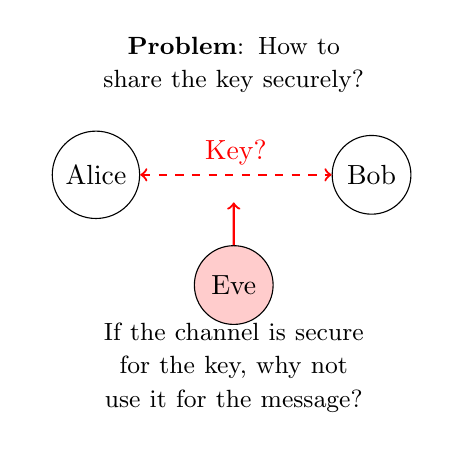
\begin{tikzpicture}[scale=0.7]
					\node[circle, draw, minimum size=1cm] (alice) at (0, 0) {Alice};
					\node[circle, draw, minimum size=1cm] (bob) at (5, 0) {Bob};
					\node[circle, draw, minimum size=1cm, fill=red!20] (eve) at (2.5, -2) {Eve};

					\draw[<->, thick, dashed, red] (alice) -- node[above] {Key?} (bob);
					\draw[->, thick, red] (eve) -- (2.5, -0.5);

					\node[text width=4cm, align=center] at (2.5, 2) {\small \textbf{Problem}: How to share the key securely?};

					\node[text width=5cm, align=center] at (2.5, -3.5) {\small If the channel is secure for the key, why not use it for the message?};
				\end{tikzpicture}
			\end{center}
		}
	\end{columns}
\end{frame}

\begin{frame}{What did the proof actually buy us?}
	\begin{itemize}[<+->]
		\item \textbf{A checklist for deployment.} Every assumption in the proof is a requirement on whoever implements it: fresh key, uniform key, attacker never tampers. Miss one and you get the attacks from the last section.
		\item \textbf{Freedom to modify.} We swapped $\oplus$ for addition mod $n$ and knew it was fine; we swapped it for $\land$ and knew it wasn't. Without the proof, both are just ``looks random to me''.
		\item \textbf{A vocabulary.} OTP is ``secure'' and ``insecure'' at the same time, depending on what you mean. Only precise definitions let us say: secrecy yes, integrity no.
		\item \textbf{A building block.} Every stream cipher in this course is ``OTP with a fake key''. We will reuse today's proof, not redo it (topic 1.4).
	\end{itemize}
\end{frame}

\begin{frame}{The provable security mindset}{What we actually did today}
	\begin{enumerate}[<+->]
		\item \textbf{Wrote the attack scenario as code.} \textsc{Attack}$(M)$: who picks what, in what order, and what the attacker gets to see.
		\item \textbf{Stated the goal as a claim about that code.} ``For every $M$, the output is uniform'', or equivalently: indistinguishable from \textsc{Junk}.
		\item \textbf{Proved it, or found the distinguisher.} XOR: exactly one key per $(M, C)$, so $1/2^n$. AND: $\textsc{Attack}(\bit{0}^n) = \bit{0}^n$, always.
		\item \textbf{Read the assumptions back as requirements.} Fresh uniform key per message; the attacker only observes.
	\end{enumerate}
	\vspace{0.5em}
	\uncover<+->{\textbf{Next time}: the same recipe with \emph{libraries} instead of a single subroutine, adversaries as \emph{programs}, and a precise definition of ``indistinguishable''.}
\end{frame}

\begin{frame}[plain]
	\titlepage
\end{frame}

\end{document}
